\section{Deutsch-Jozsa Algorithm}

\subsection{Motivation}

One interesting property of quantum circuits that we want to leverage is parallelism. This follows directly from the principle of superposition. To make it a bit more clear let us consider a black box that allows us to compute a function $f: \{0, 1\}^n \to \{0, 1\}$. We however need a place to store the result. We thus want to have a function that achieves the following operation for us,
$$ \ket{x,y} \to \ket{x, f(x)\oplus y}$$
This can be achieved with a unitary operator $U_f$. The process for constructing such an oracle would be to take the classical circuit for computing $f(x)$ and use quantum equivalents of the gates used in this circuit. Leaving aside this implementational detail we observe that if we pass in a superposition of states in $x$ in principle we can obtain multiple values of the function in a single pass.
For instance consider the simple case of $n = 1$ and suppose that
$$ x = \frac{\ket{0} + \ket{1}}{\sqrt{2}}$$

\begin{figure}[htp]
    \centering
    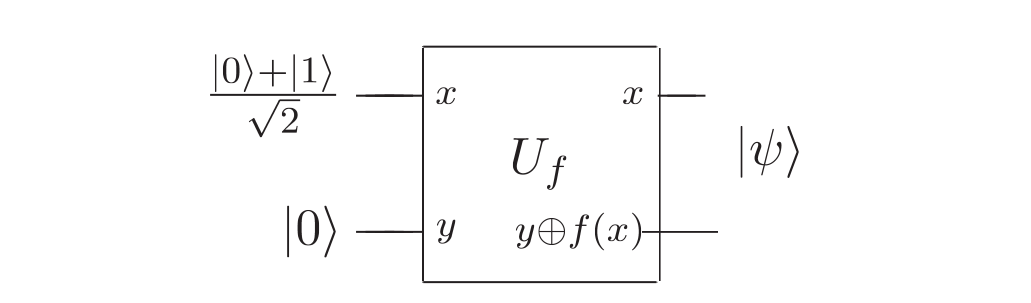
\includegraphics[width=\textwidth]{deutsch}
\end{figure}

Then the final state $\ket{\psi}$ would then be simply
$$\ket{\psi} = \frac{\ket{0, f(0)} + \ket{1, f(1)}}{\sqrt{2}}$$
This means that we have obtained two values of the function $f(x)$ by evaluating our quantum circuit just once. But unfortunately this state is a superposition. We cannot obtain both the values as measurement once collapses this state. What we therefore desire is to use this power of superposition to obtain non trivial values that would normally require us to compute the classical circuit multiple times. The Deustch Algorithm allows to find $f(0) \oplus f(1)$ by just evaluating the circuit once.

\subsection{Deustch Algorithm}

In order to obtain $f(0) \oplus f(1)$ we will use the oracle after applying the hadamard gate on the input qubits $\ket{0}$ and $\ket{1}$. This gives us a form that becomes useful in determining $f(0) \oplus f(1)$ as we will see.

Refer to the figure on the next page to see the circuit we will be implementing. 
The state $\ket{\psi_1} $ is given by
$$ \ket{\psi_1} = \frac{\ket{00} - \ket{01} + \ket{10} - \ket{11}}{2} = 
\left[\frac{\ket{0} + \ket{1}}{\sqrt{2}} \right] \left[\frac{\left{0} - \ket{1}}{\sqrt{2}}\right]$$

The state $\ket{\psi_2}$ after applying the oracle can be written in the following form 
$$\ket{\psi_2} = \pm \left[ \frac{\ket{0} + \ket{1}}{\sqrt{2}}\right]\left[\frac{\ket{0} - \ket{1}}{\sqrt{2}} \right]$$ if $f(0) = f(1)$ otherwise $$\ket{\psi_2} = \pm \left[ \frac{\ket{0} - \ket{1}}{\sqrt{2}}\right]\left[\frac{\ket{0} - \ket{1}}{\sqrt{2}} \right]$$

Observe that by applying the hadamard on the first qubit and observing that $\ket{f(0) \oplus f(1)} = \ket{0}$ if $f(0) = f(1)$ and $\ket{1}$ otherwise gives the state $\ket{\psi_3}$ as 
$$ \ket{\psi_3} = \ket{f(0) \oplus f(1)} \left[\frac{\ket{0} - \ket{1}}{\sqrt{2}} \right]$$

Now simply measuring the first qubit allows us to find $f(0) \oplus f(1)$ in one single evaluation of the quantum circuit. This is Deustch's algorithm.
\begin{figure}[htp]
    \centering
    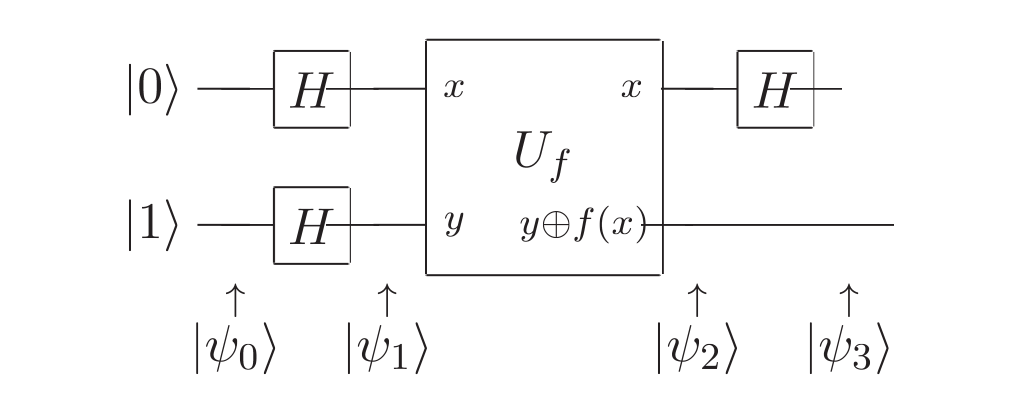
\includegraphics[width=\textwidth]{deutschcircuit}
\end{figure}

\subsection{The Deutsch-Jozsa Algorithm}

\begin{figure}[htp]
    \centering
    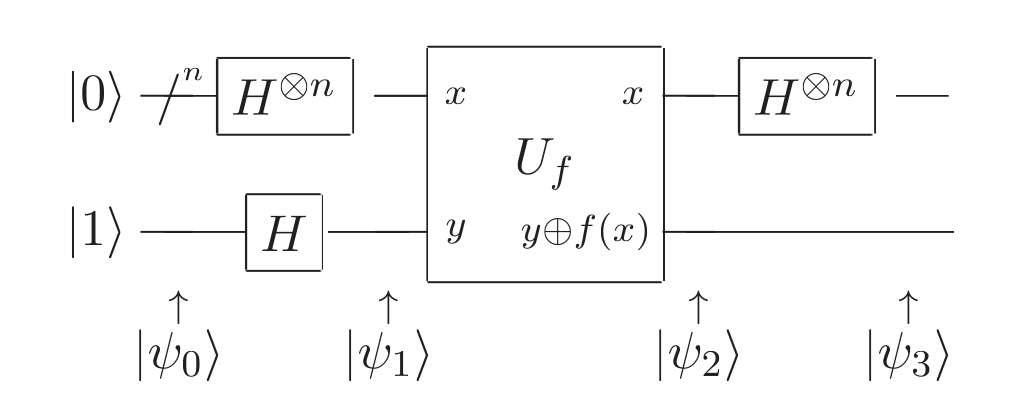
\includegraphics[width=\textwidth]{joschza}
\end{figure}

Deutsch Algorithm is a special case of the more specific Deutsch-Jozsa Algorithm. Consider the following problem which can be formulated as a game.Alice, in Amsterdam, selects a number x from $0$ to $2^n − 1$, and mails it in a letter to Bob, in Boston. Bob calculates some function
$f(x)$ and replies with the result, which is either $0$ or $1$. Now, Bob has promised to use
a function f which is of one of two kinds; either $f(x)$ is constant for all values of $x$,
or else $f(x)$ is balanced, that is, equal to $1$ for exactly half of all the possible $x$, and $0$
for the other half. Alice’s goal is to determine with certainty whether Bob has chosen a
constant or a balanced function, corresponding with him as little as possible. Classically clearly we need atleast $2^{n-1} + 1$ classical bits to resolve this. Can we do better using quantum algorithms?

It turns out we need to evaluate the oracle only once to solve this. Notice that the previous algorithm solved exactly this for the case $n=1$. Our modified oracle takes in $n$ qubits and outputs the value of $f(x)$ in the target register which we set to $\ket{1}$ initially. The circuit is shown in the previous page.

Observe that we can write $\ket{\psi_1}$ as 
$$\ket{\psi_1} = \frac{\sum_{x \in \{0, 1\}^n} \ket{x} }{\sqrt{2^n}} \left[ \frac{\ket{0} - \ket{1}}{\sqrt{2}} \right]$$

$\ket{\psi_2}$ then becomes 
$$\ket{\psi_2} = \frac{\sum_{x \in \{0, 1\}^n} (-1)^{f(x)}\ket{x} }{\sqrt{2^n}} \left[ \frac{\ket{0} - \ket{1}}{\sqrt{2}} \right]$$

Finally we apply the n gate hadamard on the first register of $n$ qubits. These qubits are already in superposition so it seems a bit complex to apply it on all of them. We can however write it as a double sum.

\begin{exercise}
Prove that $$H^{\otimes n} \ket{x_1, x_2 \cdots x_n} = \frac{\sum_{z_1, z_{2}, \cdots z_n}(-1)^{x_{1}z_{1} + x_{2}z{2} \cdots x_{n}z{n}}\ket{z_1, z_2 \cdots z_n}}{\sqrt{2^n}}$$
\end{exercise}

The above can be written simply in the form 
 $$H^{\otimes n} \ket{x} = \frac{\sum_{z}(-1)^{x.z}\ket{z}}{\sqrt{2^n}}$$ 
where $x.z$ is the bitwise product modulo 2.

Thus we can write $\ket{\psi_3}$ as
$$\ket{\psi_3} = \sum_z \sum_x \frac{\sum_{z}(-1)^{x.z + f(x)}\ket{z}}{\sqrt{2^n}}\left[\frac{\ket{0} - \ket{1}}{\sqrt{2}} \right]$$

Now suppose $f(x)$ is constant. Then we can see that the coefficient of $\ket{0}^{\otimes n}$ is either $+1$ or $-1$ depending on $f(x)$. But this means that if we measure the first $n$ qubits in the register we will obtain $\ket{0}^{\otimes n}$ with certainty as our state vector is of unit length and so the other terms have amplitude $0$. Conversely if $f(x)$ is balanced the coefficient of  $\ket{0}^{\otimes n}$ is $0$. Thus is we measure the qubits in the first register and if we obtain $\ket{0}^{\otimes n}$  we see that $f(x)$ is constant and otherwise it is balanced.

Thus using only one pass through the oracle we can solve this problem. This is far far better than the classical case where we need to evaluate the function at $2^{n-1} + 1$ values. This sums up the Deutsch-Jozsa Algorithm.